\documentclass[12pt]{article}
\usepackage{graphicx}

\title{COP290: User Registration App}
\author{Anuj Mahajan (2011CS50833) \\ Apoorva Gollapalli (2014CS50284) \\ Avinash Tantati (2014CS10259) }

\begin{document}
\maketitle

This is the description of a an android application that provides access to Moodle an educational service, The app works by using API calls to the web2py server provided. 


\begin{figure}[!ht]
	\centering
	
\includegraphics[width=0.5\textwidth]{./splash}
	\caption{Splash Page}
\end{figure}

\begin{figure}[!ht]
	\centering
	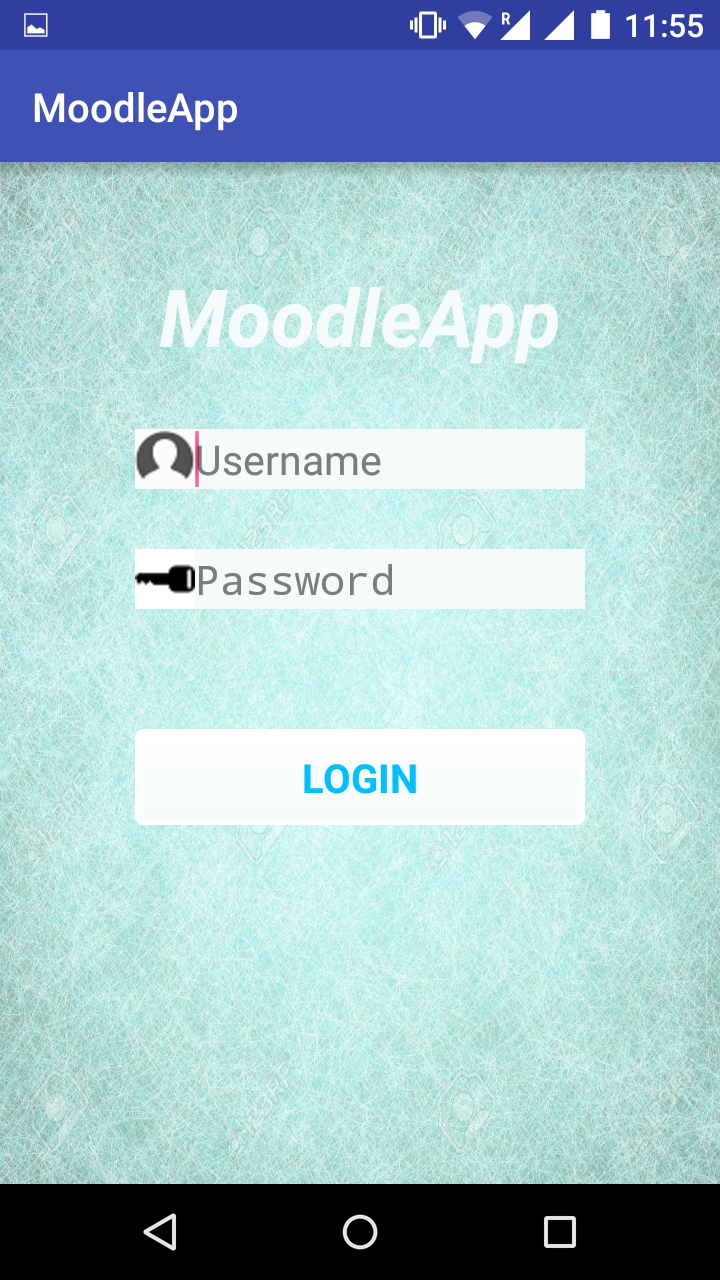
\includegraphics[width=0.5\textwidth]{./login}
	\caption{Login screen}
\end{figure}

\begin{figure}[!ht]
	\centering
	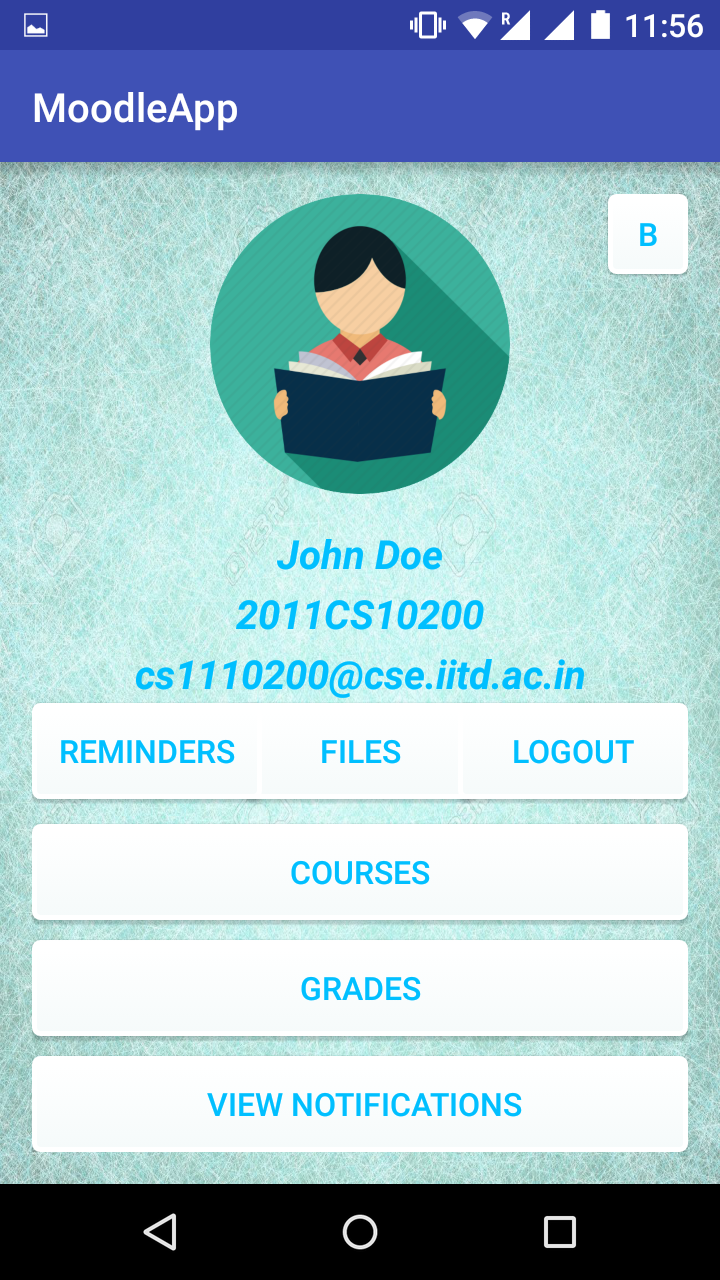
\includegraphics[width=0.5\textwidth]{./profile}
	\caption{Profile page}
\end{figure}

\begin{figure}[!ht]
	\centering
	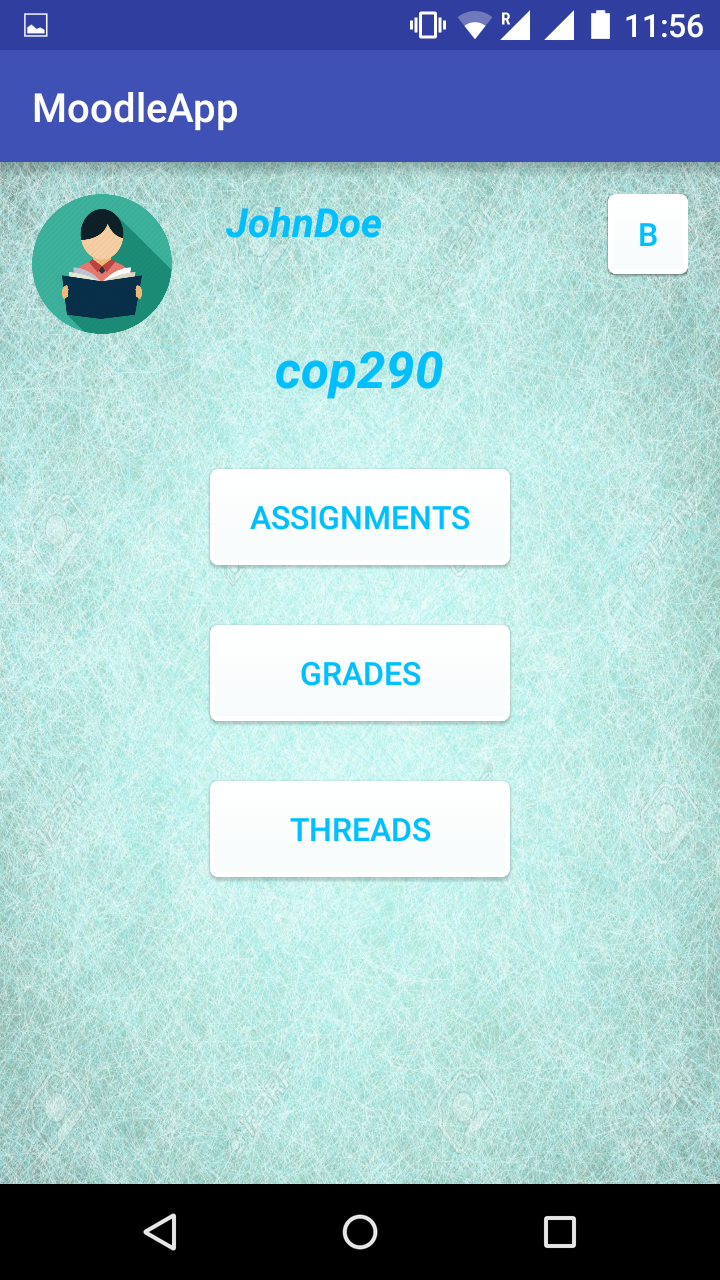
\includegraphics[width=0.5\textwidth]{./course}
	\caption{Course page}
\end{figure}

\begin{figure}[!ht]
	\centering
	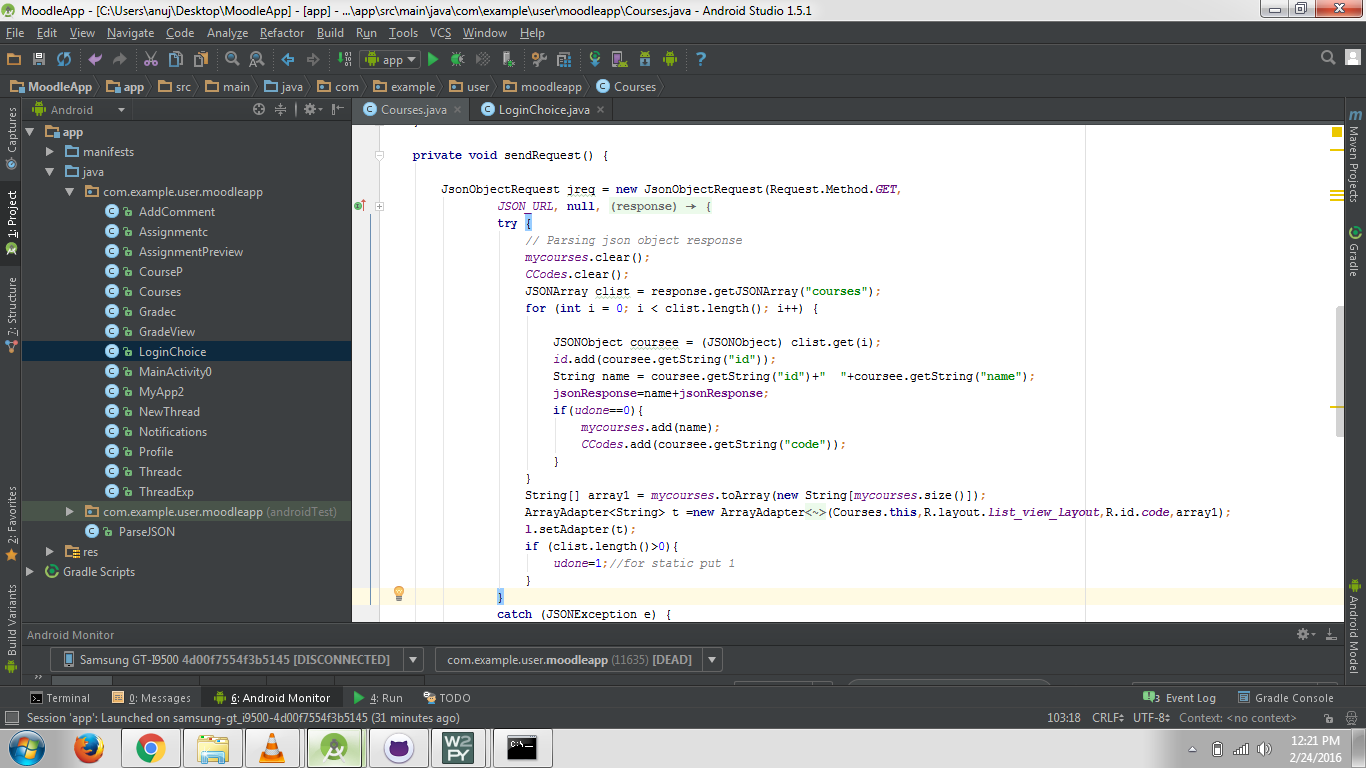
\includegraphics[width=0.5\textwidth]{./request}
	\caption{Typical Request}
\end{figure}


\begin{figure}[!ht]
	\centering
	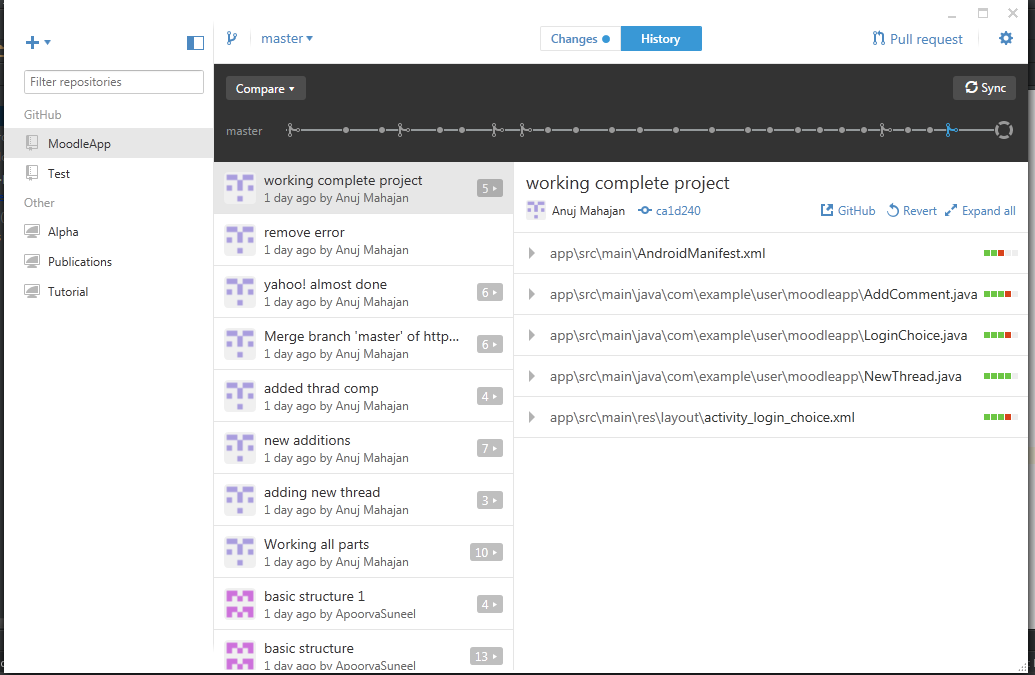
\includegraphics[width=0.5\textwidth]{./git}
	\caption{Git Commits}
\end{figure}


\section{User Interface}
\begin{itemize}
\item We have implemented multiple activities for the application, we follow a tree like stucture that mimics the web application for moodle plus with respect to the APIs provided, 

\end{itemize}

\section{Implementation Details}

\begin{itemize}
\item We have explicitly used static variables for stiring session informatio  and sharing the same across activities
\item We implemented some nice list views for the UI display
	\begin{itemize}
		\item Since the UI was desired to be used on any size of the screens we, decides to use Listview with nested tree like activity browsing instead of fragments 
		\item For dynamic updates for Threads, notifications and comments we have cleverly implemented back buttons that refetch the data using theURL request and then update the adapter for listview by clearing thr old data holder Array Lists
	\end{itemize}
\item We used the volley JSONObjectRequest request for fetching the data from the servers. We found the information provided at~\cite{volley_tutorial_1}, ~\cite{volley_tutorial_2} and ~\cite{android_network_tutorial} very useful.
\item The generic Send Request funstion was modified for various API fetchs by changing the URLs and adding proper JSON parser code with each request, We maintained the state of the application fot the child activities by using the variables like Tsel, Csel that maintained the courses selected
\item The comments and new threads generated are handled using a edit text entry that allows adding multiple items
\item We also gave our application a cool design by exploring opportunities for changing the activity backgrounds, activity icons and changing the activity and button layouts and characteristics.
\end{itemize}



The code for the project is being maintained in this repository: {\em \\https://github.com/anujmahajan/MoodleApp.git }.

\bibliographystyle{abbrv}
\bibliography{references}

\end{document}
